% figures/oracle-topology.tex
% Every correctness claim compares one semantic module executed three
% ways: GPU path, sequential CPU oracle, and PyTorch reference.
\documentclass[tikz,border=10pt]{standalone}
% figures/common-preamble.tex
% Shared setup for the TikZ documentation figures. Colors mirror the
% palette in scripts/render_docs_diagrams.py so both atlases match.
\usepackage[T1]{fontenc}
\usepackage{lmodern}
\usepackage{tikz}
\usepackage{pgfplots}
\pgfplotsset{compat=1.18}
\usetikzlibrary{arrows.meta}
\usetikzlibrary{backgrounds}
\usetikzlibrary{calc}
\usetikzlibrary{decorations.pathreplacing}
\usetikzlibrary{fit}
\usetikzlibrary{positioning}

\definecolor{swcanvas}{HTML}{FFFDF8}
\definecolor{swpanel}{HTML}{F5F3ED}
\definecolor{swink}{HTML}{17212B}
\definecolor{swmuted}{HTML}{4B5563}
\definecolor{swline}{HTML}{59636E}
\definecolor{swblue}{HTML}{00689D}
\definecolor{swbluefill}{HTML}{DCEFFD}
\definecolor{swpurple}{HTML}{8E4775}
\definecolor{swpurplefill}{HTML}{F7E2EF}
\definecolor{sworange}{HTML}{A94500}
\definecolor{sworangefill}{HTML}{FCE5DC}
\definecolor{swgreen}{HTML}{00664B}
\definecolor{swgreenfill}{HTML}{DDF4EB}
\definecolor{swgrayfill}{HTML}{EEF0F2}

\pagecolor{swcanvas}
\AtBeginDocument{\color{swink}}

\tikzset{
  swcell/.style={
    draw, minimum width=0.46cm, minimum height=0.46cm, inner sep=0pt,
    line width=0.7pt, rounded corners=1pt},
  swbox/.style={
    draw=swline, fill=swpanel, rounded corners=6pt, line width=0.9pt},
  swarrow/.style={-{Stealth[length=6pt]}, draw=swline, line width=1pt},
  swtag/.style={
    draw, rounded corners=8pt, line width=0.9pt,
    font=\bfseries\scriptsize, inner xsep=8pt, inner ysep=4pt},
  swtitle/.style={anchor=west, font=\Large\bfseries, text=swink},
  swsubtitle/.style={anchor=west, font=\small, text=swmuted},
  swcode/.style={font=\small\ttfamily, text=swink},
  every picture/.style={line cap=round},
}

\begin{document}
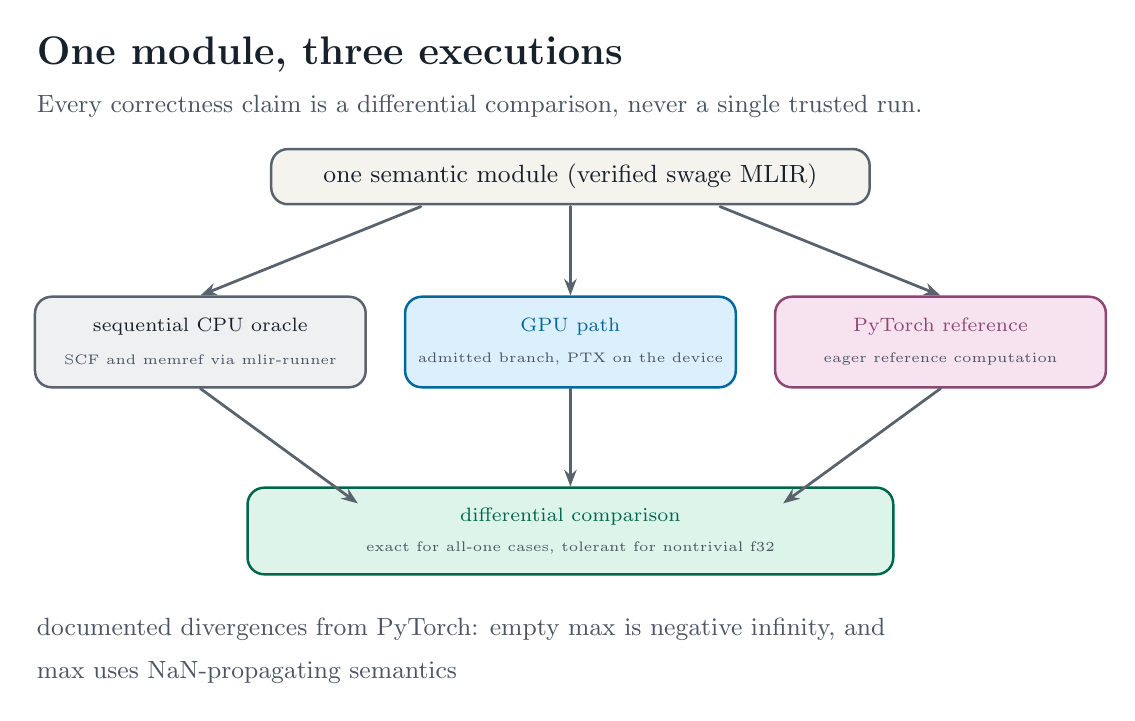
\begin{tikzpicture}[x=1cm, y=1cm]

% Header.
\node[swtitle] at (0, 1.15) {One module, three executions};
\node[swsubtitle] at (0, 0.5)
  {Every correctness claim is a differential comparison, never a
   single trusted run.};

% The shared input.
\node[swbox, minimum width=7.6cm, minimum height=0.7cm]
  (module) at (6.9, -0.4) {};
\node[font=\small, text=swink] at (6.9, -0.4)
  {one semantic module (verified swage MLIR)};

% Three executions of the same module.
\node[swbox, fill=swgrayfill, minimum width=4.2cm,
      minimum height=1.15cm] (cpu) at (2.2, -2.5) {};
\node[font=\scriptsize, text=swink] at (2.2, -2.3)
  {sequential CPU oracle};
\node[font=\tiny, text=swmuted] at (2.2, -2.72)
  {SCF and memref via mlir-runner};
\node[swbox, draw=swblue, fill=swbluefill, minimum width=4.2cm,
      minimum height=1.15cm] (gpu) at (6.9, -2.5) {};
\node[font=\scriptsize, text=swblue] at (6.9, -2.3)
  {GPU path};
\node[font=\tiny, text=swmuted] at (6.9, -2.72)
  {admitted branch, PTX on the device};
\node[swbox, draw=swpurple, fill=swpurplefill, minimum width=4.2cm,
      minimum height=1.15cm] (torch) at (11.6, -2.5) {};
\node[font=\scriptsize, text=swpurple] at (11.6, -2.3)
  {PyTorch reference};
\node[font=\tiny, text=swmuted] at (11.6, -2.72)
  {eager reference computation};
\draw[swarrow] (5.0, -0.78) -- (cpu.north);
\draw[swarrow] (6.9, -0.78) -- (gpu.north);
\draw[swarrow] (8.8, -0.78) -- (torch.north);

% The comparisons.
\node[swbox, draw=swgreen, fill=swgreenfill, minimum width=8.2cm,
      minimum height=1.1cm] (compare) at (6.9, -4.9) {};
\node[font=\scriptsize, text=swgreen] at (6.9, -4.72)
  {differential comparison};
\node[font=\tiny, text=swmuted] at (6.9, -5.12)
  {exact for all-one cases, tolerant for nontrivial f32};
\draw[swarrow] (cpu.south) -- (4.2, -4.55);
\draw[swarrow] (gpu.south) -- (gpu.south |- compare.north);
\draw[swarrow] (torch.south) -- (9.6, -4.55);

% Documented divergences from the PyTorch reference.
\node[anchor=west, font=\small, text=swmuted] at (0, -6.15)
  {documented divergences from PyTorch:
   empty max is negative infinity, and};
\node[anchor=west, font=\small, text=swmuted] at (0, -6.7)
  {max uses NaN-propagating semantics};

\end{tikzpicture}
\end{document}
